\documentclass[12pt, letterpaper]{article}

\usepackage[utf8]{inputenc}
\usepackage{float}
\usepackage{systeme}
\usepackage{amsmath}
\usepackage{amssymb}
\usepackage{enumitem}
\usepackage{amsfonts}
\usepackage{amsthm}
\usepackage{graphicx}
\usepackage[colorinlistoftodos]{todonotes}
\usepackage{pifont}
\usepackage{mdframed,color}
\usepackage[letterpaper, left=3cm, right=3cm, top=3cm, bottom=3cm]{geometry}
\newcommand{\Z}{\mathbb{Z}}
\newcommand{\N}{\mathbb{N}}
\newcommand{\C}{\mathbb{C}}
\newcommand{\Q}{\mathbb{Q}}
\newcommand{\R}{\mathbb{R}}
\newcommand{\F}{\mathbb{F}}
\newtheoremstyle{statement}{3pt}{3pt}{}{}{\bfseries}{:}{.5em}{}

\theoremstyle{statement}
\newtheorem*{atmProp}{Proposition}

\theoremstyle{statement}
\newtheorem*{atmStat}{Statement}

\newenvironment{atmProof}{\noindent\ignorespaces\paragraph{Proof:}}{\hfill \ding{122}\par\noindent}

\newenvironment{Solution}{\noindent\ignorespaces\paragraph{Solution:}}{\hfill \ding{122}\par\noindent}

\newcount\arrowcount
\newcommand\arrows[1]{
        \global\arrowcount#1
        \ifnum\arrowcount>0
                \begin{matrix}
                \expandafter\nextarrow
        \fi
}

\newcommand\nextarrow[1]{
        \global\advance\arrowcount-1
        \ifx\relax#1\relax\else \xrightarrow{#1}\fi
        \ifnum\arrowcount=0
                \end{matrix}
        \else
                \\
                \expandafter\nextarrow
        \fi
}

\title{Mastery Homework 4}
\author{Rafael Laya}
\date{Fall 2018}

\begin{document}
    \maketitle
    
    \section*{Section 1.9}
    \subsection*{Problem 26}
    \begin{atmStat}
    Determine if the linear transformation $\operatorname{T}$ is a) One to One b) onto. With
    $\operatorname{T}:\R^3\longrightarrow\R^2$, $\operatorname{T}(\Vec{e_1})=(1, 3), \operatorname{T}(\Vec{e_2})=(4,-7),$ and $\operatorname{T}(\Vec{e_3})=(-5, 4)$ and where $\Vec{e_1}, \Vec{e_2}, \Vec{e_3}$ are the columns of the identity matrix.
    \end{atmStat}
    \begin{Solution}
    
    a) The linear transformation $\operatorname{T}$ is One to One if and only if the equation $\operatorname{T}(\Vec{x})=\Vec{0}$ only has trivial solution. Given the information in the statement we know the standard matrix $A$ of the linear transformation: 
    
    $$
    A = \begin{bmatrix}
    1 & 4 & -5 \\
    3 & -7 & 4
    \end{bmatrix}
    $$
    
    Then, $\operatorname{T}(\Vec{x})=A\Vec{x}=\Vec{0}$ can be solved by row reducing the augmented matrix $\begin{bmatrix} A && \Vec{0}\end{bmatrix}$
    
    $$
    \begin{bmatrix}
    1 & 4 & -5 && 0\\
    3 & -7 & 4  && 0
    \end{bmatrix}
    $$
    
    Notice, however, that $A$ has two rows and three columns, therefore it can have at most two pivots (one pivot per row). If $A$ has at most two pivot columns then the system is either inconsistent (which is false since $A\Vec{x}=\Vec{0}$ always has trivial solution) or there is a free variable in the linear system with augmented matrix $\begin{bmatrix}A&&\Vec{0} \end{bmatrix}$ and therefore there are infinitely many solutions. If there are infinitely many solutions then we have non-trivial solutions to $\operatorname{T}(\Vec{x})=\Vec{0}$ and so $\operatorname{T}$ is not One to One.\\
    
    
    b) The linear transformation $T$ is Onto if and only if the columns of the matrix $A$ span $R^2$. Let $\Vec{b}=\begin{bmatrix}b_1\\b_2\end{bmatrix}\in\R^2$ and then we only have to row reduce $\begin{bmatrix} A && \Vec{b}\end{bmatrix}$ which is equivalent to solving the equation $x_1a_1+x_2a_2+x_3a_3=\Vec{b}$ 
    
    $$
    \begin{bmatrix}
    1 & 4 & -5 & b_1 \\
    3 & -7 & 4 & b_2
    \end{bmatrix}
    \arrows2{}{R_2-3R_1}
    \begin{bmatrix}
    1 & 4 & -5 & b_1 \\
    0 & -19 & 19 & -3b_1+b_2
    \end{bmatrix}
    \arrows2{}{-\frac{1}{19}R_2}
    \begin{bmatrix}
    1 & 4 & -5 & b_1 \\
    0 & 1 & -1 & \frac{3}{19}b_1-\frac{1}{19}b_2
    \end{bmatrix}
    $$
    
    We do not have to reach the row reduced echelon form since at this stage we know we have one pivot in every row of $A$ and therefore the right-most column of the augmented matrix cannot be a pivot column and the system is always consistent for any $\Vec{b}$. The linear transformation $\operatorname{T}$ is onto. 
    
    \end{Solution}
    \subsection*{Problem 28}
    \begin{atmStat}
    Determine if the linear transformation $\operatorname{T}$ is a) One to One b) onto.
    
    \begin{figure}[H]
        \centering
        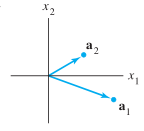
\includegraphics[scale=1.0]{Capture}
        \caption{The columns of the Standard Matrix $A$ of the linear transformation $\operatorname{T}$}
        \label{fig:fig1}
    \end{figure}
    \end{atmStat}
    \begin{Solution}
    
    a) Since the image shows that $\Vec{a_1}, \Vec{a_2}$ are not multiples of each others then the set $\{\Vec{a_1}, \Vec{a_2}\}$ is a linearly independent set. The linear transformation $\operatorname{T}$ is (by theorem) one to one if and only if the columns of $A$ are linearly independent, which is the case here. $\operatorname{T}$ is a one to one linear transformation.
    
    b) Since $\operatorname{T}:\R^2\longrightarrow\R^2$ the matrix $A$ has two columns and two rows. Since the columns of $A$ are linearly independent then $A$ has two pivots, therefore each row of $A$ has a pivot and by theorem the columns of $A$ span $\R^2$. Because the columns of $A$ span $\R^2$, again by theorem, $\operatorname{T}$ is onto.
    
    \end{Solution}
    \subsection*{Problem 34}
    \begin{atmStat}
    Why is the question "Is the linear transformation $\operatorname{T}$ onto? an existence question?
    \end{atmStat}
    \begin{Solution}
    Let $\operatorname{T}:\R^n\longrightarrow\R^m$ be a linear transformation. The question whether $\operatorname{T}$ is onto is an existence question because it is equivalent (by definition) to asking that if for every $\Vec{b}\in\R^m$ there EXISTS some $\Vec{x}\in\R^n$ such that $\operatorname{T}(\Vec{x})=\Vec{b}$ 
    \end{Solution}
    
    \section*{Section 2.1}
    \subsection*{Problem 22}
    \begin{atmStat}
    Show that if the columns of $B$ are linearly dependent, then so are the columns of $AB$.
    \end{atmStat}
    \begin{Solution}
    Let $A$ be a matrix of order mxn and $B$ of order nxp. Let $\operatorname{col_i}(M)$ be the notation for the $i$th column of a matrix $M$. Suppose the columns of $B$ are linearly dependent, that is, there is non-trivial solution $(x_1, \dots, x_p)=(c_1, \dots, c_p)$ to the equation:
    $$
    x_1\operatorname{col_1}(B)+\dots+x_p\operatorname{col_p}(B)=\Vec{0}
    $$
    Which is equivalent to having a non-trivial solution $\Vec{x}=\Vec{c}=\begin{bmatrix}c_1 \\ \vdots \\ c_p\end{bmatrix}$ to: $B\Vec{x}=\Vec{0}$. Now, multiply by $A$ on the left and apply properties of matrix multiplication:
    \begin{align*}
         B\Vec{c} &= \Vec{0} \\
         A(B\Vec{c}) &= A\Vec{0} \\
         (AB)\Vec{c} &= \Vec{0} 
    \end{align*}
    Therefore there is a non-trivial solution $\Vec{c}$ to the equation $(AB)\Vec{x}=\Vec{0}$ which is equivalent to a non-trivial solution $(x_1,\dots,x_p)=(c_1,\dots,c_p)$ to: 
    $$
    x_1\operatorname{col_1}(AB)+\dots+x_p\operatorname{col_p}(AB)=\Vec{0}
    $$
   Therefore the columns of $AB$ are linearly dependent.
    \end{Solution}
    
    \section*{Section 2.2}
    \subsection*{Problem 14}
    \begin{atmStat}
    Suppose $(B - C)D=0$ where $B$ and $C$ are mxn matrices and $D$ is invertible. Show that $B=C$.
    \end{atmStat}
    \begin{Solution}
    Take the original equation and multiply by the inverse of $D$, $D^{-1}$ on the right (in order to get, say, "rid" of $D$).
    \begin{align*}
        (B - C)D &= 0 \\
        ((B - C)D)D^{-1} &= 0D^{-1} \\
        (B - C)(DD^{-1}) &= 0 \\
        (B - C)I_n &= 0 \\
        B - C &= 0\\
    \end{align*}
    Add $C$ and then:
    \begin{align*}
        (B - C) + C &= 0 + C \\ 
        B + (-C + C) &= C \\
        B + 0 &= C \\
        B &= C
    \end{align*}
    Which is exactly what we wanted to show.
    
    \end{Solution}
    \subsection*{Problem 15}
    \begin{atmStat}
    Suppose $A, B, C$ are invertible matrices of nxn. Show that $ABC$ is also invertible by producing a matrix $D$ such that $(ABC)D=I$ and $D(ABC)=I$ 
    \end{atmStat}
    \begin{Solution}
    Recall that: $(AB)^{-1}=B^{-1}A^{-1}$. We can apply this property multiple times to figure out $D$: 
    \begin{align*}
    (ABC)^{-1} &= C^{-1}(AB)^{-1}\\
    &= C^{-1}B^{-1}A^{-1}
    \end{align*}
    So let $D=C^{-1}B^{-1}A^{-1}$ and then:
    \begin{align*}
        (ABC)D &= (ABC)(C^{-1}B^{-1}A^{-1}) \\
        &= (AB)(CC^{-1})(B^{-1}A^{-1}) \\
        &= (AB)(I)(B^{-1}A^{-1} \\
        &= (AB)(B^{-1}A^{-1} \\
        &= A(BB^{-1})A^{-1} \\
        &= (AI)A^{-1} \\
        &= AA^{-1} \\
        &= I
    \end{align*}
    And, 
    \begin{align*}
        D(ABC) &= (C^{-1}B^{-1}A^{-1})(ABC) \\
        &= (C^{-1}B^{-1})(A^{-1}A)(BC) \\
        &= (C^{-1}B^{-1})(I)(BC) \\
        &= (C^{-1}B^{-1})(BC) \\
        &= C^{-1}(B^{-1}B)C \\
        &= C^{-1}(I)C \\
        &= C^{-1}C \\
        &= I
    \end{align*}
    Therefore $ABC$ is invertible and $D= C^{-1}B^{-1}A^{-1} = (ABC)^{-1}$
    
    \end{Solution}
    \subsection*{Problem 20}
    \begin{atmStat}
    Suppose $A, B$ and $X$ are nxn matrices with $A, X$ and $A - AX$ invertible, and suppose $(A-AX)^{-1}=X^{-1}B$. a) Explain why $B$ is invertible. b) Solve for $X$. If you need to invert a matrix explain why it is invertible.
    \end{atmStat}
    \begin{Solution}
    a) By assumption $A, X$ and $A - AX$ are invertible. We can multiply by $X$ on the left (since $(X^{-1})^{-1}=X$) and this will tell us $B$ in terms of $(A-AX)^{-1}$ and $X$, all of which exist: 
    \begin{align*}
        (A-AX)^{-1}&=X^{-1}B\\
        X(A-AX)^{-1}&=X(X^{-1}B)\\
        X(A-AX)^{-1}&=(XX^{-1})B\\
        X(A-AX)^{-1}&=IB\\
        X(A-AX)^{-1}&=B
    \end{align*}
    Since $X$ is invertible and so is $(A-AX)^{-1}$ (the inverse of the inverse is the original) then by theorem, the product of two invertible matrices, $B$, is also invertible. In fact its inverse is the product of the inverses in opposite order ($B^{-1}=(A-AX)X^{-1}$)
    
    b) In order to solve for $X$ first take inverse on both sides (which is possible since the product of two invertible matrices is invertible by theorem). $B$ is invertible by part (a), and $(A-AX)^{-1}, X^{-1}$ are invertible since $A-AX, X$ are invertible by assumption and the inverse of the inverse is the original,
    
    \begin{align*}
        (A-AX)^{-1}&=X^{-1}B \\
        ((A-AX)^{-1})^{-1} &= B^{-1}(X^{-1})^{-1} \\
        A-AX &= B^{-1}X
    \end{align*}
    Add $AX$ to both sides,
    \begin{align*}
        A-AX+AX&=B^{-1}X+AX \\
        A &= (B^{-1}+A)X \\
    \end{align*}
    Since $A$ is invertible then $(B^{-1}+A)X$ must be invertible (they are equal). We know by assumption $X$ is invertible and then the other factor must be invertible (because we can multiply by $X^{-1}$ on the right and $AX^{-1}$ is the product of two invertible matrices and therefore $(B^{-1}+A)=AX^{-1}$ is invertible too). Multiply by $(B^{-1}+A)^{-1}$ on the left,
    \begin{align*}
        (A+B^{-1})^{-1}A&=(A+B^{-1})^{-1}(A+B^{-1})X \\
        (A+B^{-1})^{-1}A &= IX \\
        (A+B^{-1})^{-1}A &= X \\
    \end{align*}
    Which is what we wanted (to solve for $X$).
    \end{Solution}
    
\end{document}
